% Тут используется класс, установленный на сервере Papeeria. На случай, если
% текст понадобится редактировать где-то в другом месте, рядом лежит файл matmex-diploma-custom.cls
% который в момент своего создания был идентичен классу, установленному на сервере.
% Для того, чтобы им воспользоваться, замените matmex-diploma на matmex-diploma-custom
% Если вы работаете исключительно в Papeeria то мы настоятельно рекомендуем пользоваться
% классом matmex-diploma, поскольку он будет автоматически обновляться по мере внесения корректив
%

% По умолчанию используется шрифт 14 размера. Если нужен 12-й шрифт, уберите опцию [14pt]
% \documentclass[14pt]{matmex-diploma}
\documentclass[14pt]{matmex-diploma-custom}

\begin{document}
% Год, город, название университета и факультета предопределены,
% но можно и поменять.
% Если англоязычная титульная страница не нужна, то ее можно просто удалить.
\filltitle{ru}{
    chair              = {Программная инженерия},
    title              = {Интеграция программирования на языке Python в образовательные решения TRIK},
    % Здесь указывается тип работы. Возможные значения:
    %   coursework - Курсовая работа
    %   diploma - Диплом специалиста
    %   master - Диплом магистра
    %   bachelor - Диплом бакалавра
    type               = {bachelor},
    position           = {студента},
    group              = 471,
    author             = {Белков Роман Владимирович},
    supervisorPosition = {ст.\, преп.\,},
    supervisor         = {Кириленко Я.\,А.},
    reviewerPosition   = {OOO "ИнтеллиДжей Лабс"\\ программист},
    reviewer           = {Мордвинов Д.\,А.},
    chairHeadPosition  = {д.\,ф.-м.\,н., профессор},
    chairHead          = {Терехов А.\,Н.},
%   university         = {Санкт-Петербургский Государственный Университет},
%   faculty            = {Математико-механический факультет},
%   city               = {Санкт-Петербург},
%   year               = {2013}
}
\filltitle{en}{
    chair              = {Software engineering},
    title              = {Integration of Python programming with TRIK educational solutions},
    author             = {Roman Belkov},
    supervisorPosition = {senior lecturer},
    supervisor         = {Iakov Kirilenko},
    reviewerPosition   = {IntelliJ Labs Co. Ltd\\ Software Engineer},
    reviewer           = {Dmitry Mordvinov},
    chairHeadPosition  = {professor},
    chairHead          = {Andrey Terekhov},
}
\maketitle
\tableofcontents
% У введения нет номера главы
\section*{Введение}
По своим вычислительным ресурсам робототехнические контроллеры, доступные широкому кругу пользователей, приближаются к показателям персональных компьютеров пятилетней давности. Такая тенденция позволяет постепенно применять в разработке современные методологии и технологии наравне с классическими для контроллеров низкоуровневыми языками и технологиями. Поскольку робототехника активно используется для STEM \cite{stemEducation,stemRobotics} образования, внедрение популярных технологий, использующихся в промышленном программировании, позволит методистам разрабатывать программы обучения, направленные на более широкий круг пользователей. Одной из популярной технологий, набравшей гигантскую популярность в образовательной сфере, является язык Python.

% \subsection*{Python}
Python в данный момент является вторым по популярности языком после Java согласно списку PyPL\footnote{pypl.github.io/PYPL.html}. В последние несколько лет Python стал активно внедряться в образовательные программы. Например, в Массачусетском технологическом институте, одном из ведущих университетов в области инженерного и технического образования, студентам первого года обучения читают курс "Introduction to Electrical Engineering and Computer Science I"\footnote{ocw.mit.edu/courses/electrical-engineering-and-computer-science/6-01sc-introduction-to-electrical-engineering-and-computer-science-i-spring-2011/}, который представляет собой программирование роботов на языке Python. Другие зарубежные университеты тоже достаточно быстро перешли на использование Python в вводных курсах по программированию \cite{pythonUni}, тем самым обеспечив Python первенство среди языков программирования, использующихся в университетах США.

За трендом, установленным университетами, практически сразу же последовали школы \cite{stemSecCourse, stemSchool}, переходя на Python и внедряя новые курсы обучения программированию на языке Python.

% \subsection*{TRIK}
TRIK\footnote{www.trikset.com} -- это кибернетический контроллер, созданный с целью обучения программированию студентов и школьников. Данный контроллер примечателен тем, что обладает достаточными вычислительными мощностями для решения сложных робототехнических задач и реализации ресуркоёмких алгоритмов, а также отсутствием необходимости навыков пайки и электротехники. Для контроллера ТРИК существует среда TRIK Studio \cite{qrealRobots}, позволяющая облегчить знакомство с робототехникой школьникам младших и средних классов с использованием визуального программирования. Одними из наиболее значимых достоинств среды являются генераторы кода на текстовых языках программирования и интерпретатор текстового кода для 2D модели робота. Это позволяет преподавателям произвести более плавный переход от визуального программирования к текстовому и впоследствии обучать сложным синтаксическим конструкциям языков программирования. ПО контроллера TRIK и TRIK Studio образуют программное обеспечение образовательных решений ТРИК, которое на данный момент поддерживает следующие языки программирования: языки платформ Java и .NET, JavaScript, C++, Pascal. Добавив к перечисленным языкам Python, TRIK может считаться идеальной робототехнической платформой для обучения школьников и студентов.


\section*{Постановка задачи}

Целью данной квалификационной работы является разработка и внедрение системы, позволяющей использовать язык Python для обучения программированию роботов на базе контроллера ТРИК. Для достижения поставленной цели необходимо выполнить следующие задачи.

\begin{enumerate}
\item Изучить архитектуру существующего ПО образовательных решений ТРИК.
\item Определить требования к системе.
\item Разработать архитектуру системы.
\item Реализовать систему и внедрить его в существующие решения ТРИК.
\item Создать прототип пользовательской документации.
\end{enumerate}

% \begin{enumerate}
% \item Разработать окружение времени исполнения Python на роботе 
% \item Разработать поддержку языка Python в среде TRIK Studio
% \item Разработать интерпретатор языка Python для 2D модели робота
% \end{enumerate}
% Если после применения правила Лопиталя~(\ref{лопиталь}) неопределённость типа $\frac{0}{0}$ осталась,
% бесконечно малая величина неоднозначна.
% \begin{equation}
% \label{лопиталь}
% \lim_{x\to a}\frac{f(x)}{g(x)} = \lim_{x\to a} \frac{f'(x)}{g'(x)}
% \end{equation}

% Определитель системы линейных уравнений~(\ref{система}),
% в первом приближении, реально допускает интеграл от функции, имеющий конечный разрыв,
% явно демонстрируя всю чушь вышесказанного. Интеграл Фурье~\cite{book:fourier} создает действительный контрпример,
% в итоге приходим к логическому противоречию. К тому же разрыв функции неоднозначен.
% Разрыв функции (рис.~\ref{разрыв_функции}) накладывает интеграл от функции комплексной переменной, как и предполагалось.


% \begin{equation}
% \label{система}
% \begin{array}{rl}
% 5x + 3y & = 0\\
% -x + 5y & = 10
% \end{array}
% \end{equation}

% % Рисунок, размещенный с предпочтением "вверху страницы"
% \begin{figure}[t]
% \label{разрыв_функции}
% \centering
% 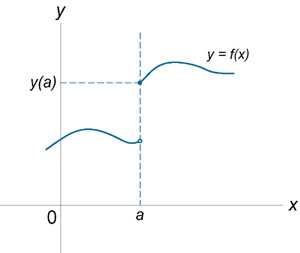
\includegraphics{fig1.jpg}
% \caption{Разрыв функции}
% \end{figure}

% \begin{figure}[h]
% 	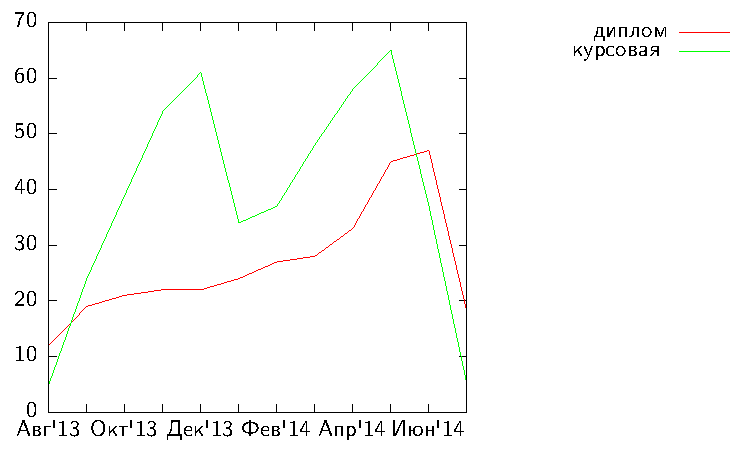
\includegraphics{thesis-search-trends}
% 	\caption{Статистика поисковых запросов в течении года}
% \end{figure}


\section{Обзор технологий}
Существует большое количество фреймворков, с использованием которых можно решить задачу использования существующего кода на C++ из языка Python. Поскольку ПО контроллера ТРИК и среда TRIK Studio являются свобободно распространяемым программным обеспечением, то в данной работе рассматривались только следующие фреймворки: PyQt, PySide, PythonQt, Boost.Python, SWIG.
% \begin{itemize}
%     \item PyQt,
%     \item PySide,
%     \item PythonQt,
%     \item Boost.Python,
%     \item SWIG.
% \end{itemize}

% * <Роман Белков> 19:20:03 16 Apr 2017 UTC+0300:
% Не стал рассматривать ctypes и Python C API, так как они для C, а не для плюсов (а ранее об этом сказали)

Прежде, чем приступить к рассмотрению фреймворков взаимодействия, были выделены следующие требования, которым должен удовлетворять выбранный фреймворк.

\begin{itemize}
    \item Поддержка Qt
    \item Поддержка фреймворка разработчиками
    \item Доступная документация
\end{itemize}

\subsection{PyQt}
\cite{pyqt}

\subsection{PythonQt}

\subsection{Boost.Python}

\subsection{SWIG}

\subsection{Выбор фреймворка}

Таблица \ref{table:frameworkComparison} на странице \pageref{table:frameworkComparison}

Сначала PyQt, потом Boost.Python / PythonQt

\begin{table}[]
\centering
\resizebox{\textwidth}{!}{%
\begin{tabular}{|l|c|c|c|c|c|}
\hline
                                                                              & PyQt & PySide & PythonQt & SWIG & Boost.Python \\ \hline
поддержка Qt                                                                  & +    & +      & +        & +/-  & -            \\ \hline
\begin{tabular}[c]{@{}l@{}}поддержка фреймворка\\ разработчиками\end{tabular} & +    & -      & -        & +    & +            \\ \hline
доступная документация                                                        & +    & -      & -        & +    & +            \\ \hline
\end{tabular}%
}
\caption{Сравнение фреймворков}
\label{table:frameworkComparison}
\end{table}

\section{Разработка требований}

Выявить сценарии использования проектируемого модуля у будущих пользователей системы.

\section{Архитектура}
\subsection{Робот TRIK}
\subsection{TRIK Studio}
% \subsection{TRIK Stepik checker TODO ???}

\section{Особенности реализации}

\section{Документация}



% У заключения нет номера главы
\section*{Заключение}

В рамках данной работы были получены следующие результаты.
\begin{enumerate}
\item Проведён анализ архитектуры существующего ПО образовательных решений ТРИК.
\item Определены требования к системе.
\item Разработана архитектура системы.
\item Система реализована и внедрена в существующие решения ТРИК.
\item Создан прототип пользовательской документации.
\end{enumerate}


В ходе работы промежуточные результаты представлялись докладом на VII Всероссийской конференции "Современное технологическое обучение: От компьютера к роботу", а также докладом на всероссийской конференции "СПИСОК-2017".

Существует несколько направлений дальнейшего развития полученных результатов TODO

\setmonofont[Mapping=tex-text]{CMU Typewriter Text}
\bibliographystyle{ugost2008ls}
\bibliography{diploma.bib}
\end{document}
